\subsection{Power capping come tecnica di controllo energetico}
\label{subsec:power_capping}

Una delle tecniche più consolidate per la gestione del consumo energetico
nei sistemi di calcolo distribuiti è il \emph{power capping}, ovvero
l'imposizione di un limite superiore alla potenza assorbita da uno o
più componenti dell'infrastruttura. A differenza degli approcci orientati
all'ottimizzazione dell'efficienza energetica in senso \emph{best-effort},
il power capping introduce il consumo di potenza come vincolo operativo
esplicito (\emph{hard constraint}), che il sistema non deve violare
durante l'esecuzione dei carichi di lavoro. L'adozione di tali meccanismi
è motivata da vincoli infrastrutturali concreti: i limiti fisici
dell'impianto elettrico, le capacità massime dei sistemi di raffreddamento
o la necessità di operare con budget energetici limitati, come in scenari
Edge o IoT. In letteratura, il problema è classicamente formulato come
un'ottimizzazione vincolata, in cui l'obiettivo consiste nel massimizzare
le prestazioni complessive del sistema nel rispetto di un budget di
potenza prefissato $P_{\max}$.

\subsubsection{Applicabilità degli approcci tradizionali nel contesto serverless}

Approcci consolidati, come quelli analizzati da Ciesielczyk et
al.~\cite{Ciesielczyk2021}, sfruttano leve hardware quali il
\emph{Dynamic Voltage and Frequency Scaling} (DVFS) o interfacce dedicate
come Intel RAPL per modulare dinamicamente la frequenza dei processori e
limitare il consumo di potenza. Tali tecniche si sono dimostrate efficaci
in contesti HPC e in data center tradizionali, operando prevalentemente a
livello di nodo fisico con una granularità temporale relativamente
grossolana.

L'applicazione di questi meccanismi al paradigma serverless introduce
tuttavia criticità specifiche. La natura effimera, \emph{stateless} e
altamente granulare delle funzioni FaaS rende le politiche di capping
statiche spesso poco reattive rispetto alla forte variabilità del carico
di lavoro. Inoltre, il disaccoppiamento tra l'esecuzione delle funzioni e
la gestione diretta delle risorse hardware limita la possibilità di
applicare controlli di potenza con una precisione coerente con la scala
temporale delle invocazioni serverless.

\subsubsection{Impatto sulle prestazioni e approcci adattivi}

L'imposizione di vincoli di potenza in ambienti serverless può comportare
degradazioni delle prestazioni non lineari, riconducibili a due categorie
di effetti ben documentate in letteratura~\cite{Qiu2023PARM}.

La prima riguarda la latenza delle funzioni: esiste una correlazione
diretta tra la riduzione della frequenza della CPU, indotta dal power
capping, e l'aumento della latenza \emph{end-to-end}. Tale effetto è
particolarmente marcato per workload \emph{CPU-bound}, mentre le funzioni
\emph{I/O-bound} risultano meno sensibili, poiché il tempo di esecuzione
è dominato da operazioni di attesa piuttosto che di elaborazione.

La seconda criticità riguarda l'interazione con le politiche di
autoscaling basate su metriche di utilizzo. In presenza di throttling
energetico, il rallentamento dell'esecuzione viene spesso interpretato
come un incremento del carico, inducendo decisioni di scaling subottimali.
Questo comportamento è particolarmente problematico in sistemi adattivi,
dove la non-stazionarietà introdotta dal vincolo di potenza può
compromettere l'efficacia dei meccanismi di apprendimento e di controllo.
La Tabella~\ref{tab:power_capping_effects} sintetizza questi effetti,
evidenziandone l'intensità differenziata in funzione del tipo di workload
e della politica di gestione delle risorse considerata.

\begin{table}[ht]
    \centering
    \caption{Sintesi degli effetti del power capping sulle prestazioni in
    ambienti serverless (rielaborazione basata su~\cite{Qiu2023PARM}).}
    \label{tab:power_capping_effects}
    \renewcommand{\arraystretch}{1.3}
    \begin{tabular}{@{}lp{6cm}l@{}}
        \toprule
        \textbf{Ambito} & \textbf{Effetto osservato} &
        \textbf{Intensità impatto} \\ \midrule
        Latenza CPU-bound & Aumento quasi lineare rispetto alla riduzione
        di frequenza. & Alto \\
        Latenza I/O-bound & Impatto marginale, limitato alle fasi di
        elaborazione. & Basso \\
        Autoscaling & Decisioni subottimali dovute a metriche non
        stazionarie. & Critico \\
        SLO & Incremento delle violazioni degli accordi di servizio.
        & Critico \\ \bottomrule
    \end{tabular}
\end{table}

Per mitigare questi effetti, Qiu et al. propongono PARM
(\emph{Adaptive Resource Allocation for Datacenter Power
Capping})~\cite{Qiu2023PARM}, un framework adattivo che interviene sulla
catena decisionale dell'autoscaling in presenza di vincoli di potenza
attivi. Come illustrato in Figura~\ref{fig:parm_architecture}, PARM
introduce un ciclo di controllo che opera in coordinamento con il
meccanismo di power capping fisico, articolato in due componenti
principali: un \emph{Degradation Predictor}, che stima a runtime
l'impatto del throttling sulle prestazioni applicative, e un
\emph{Resource Re-allocator}, che intercetta e corregge le decisioni
dell'autoscaler prima che vengano applicate al livello di orchestrazione.

\begin{figure}[ht]
    \centering
    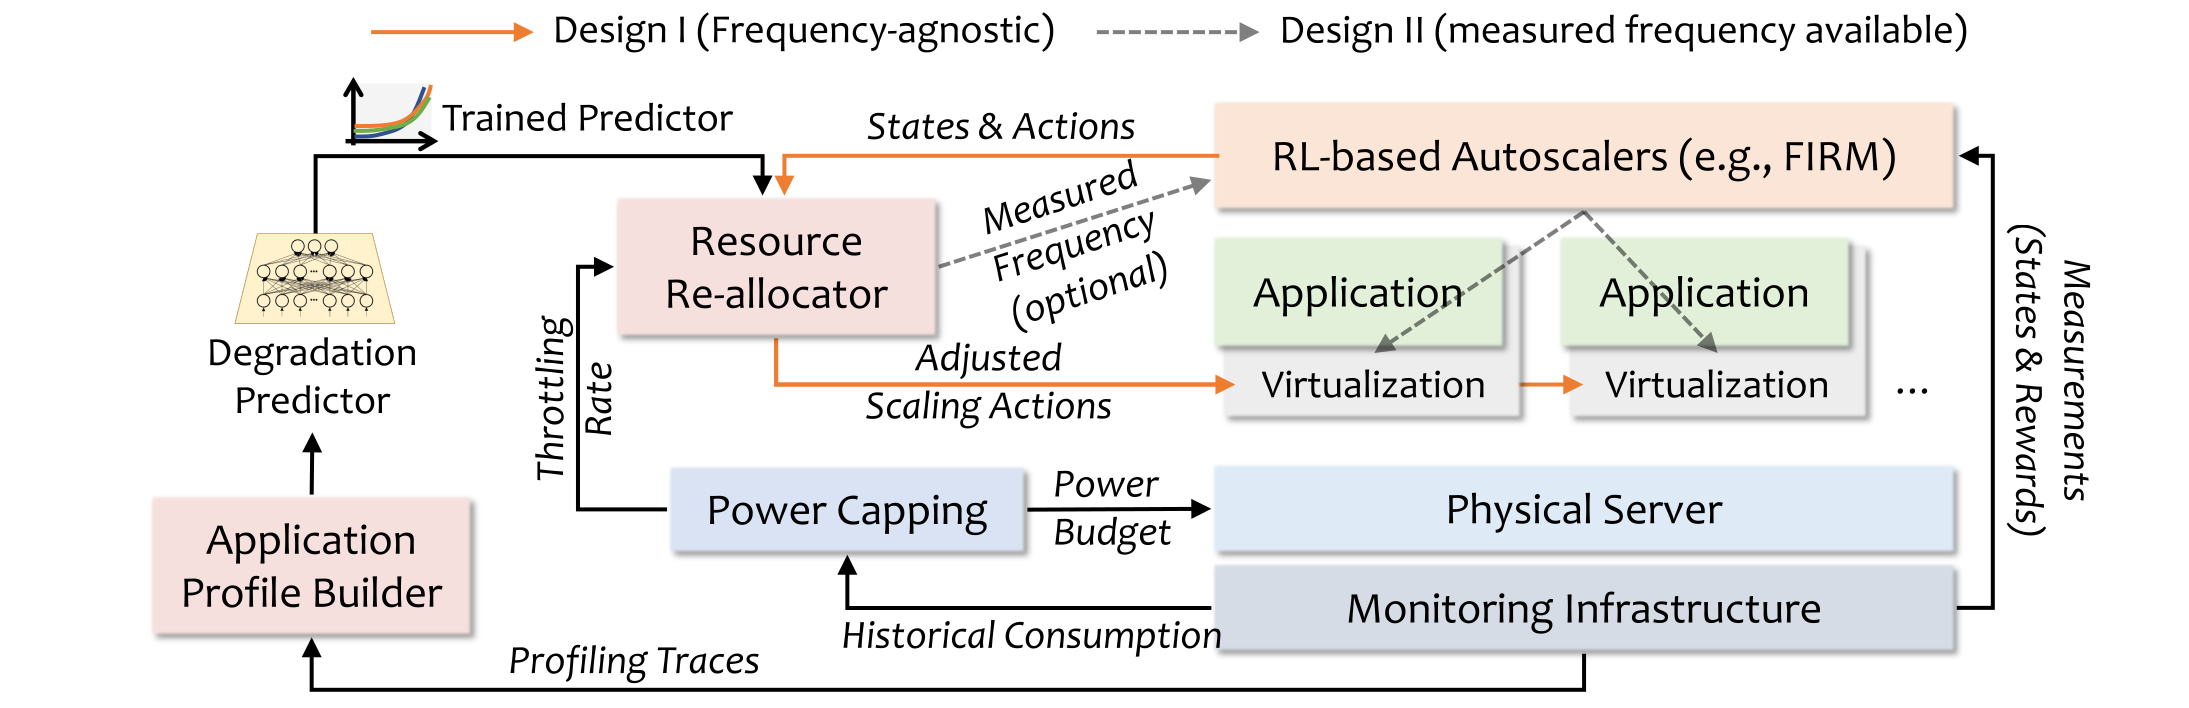
\includegraphics[width=0.9\textwidth]{figures/parm_architecture.png}
    \caption{Schema architetturale del framework PARM. Il
    \emph{Degradation Predictor} stima l'impatto del power capping sulle
    prestazioni, mentre il \emph{Resource Re-allocator} adatta
    dinamicamente le decisioni di scaling in presenza di vincoli di
    potenza.}
    \label{fig:parm_architecture}
\end{figure}

Nel complesso, il power capping rappresenta un meccanismo efficace per
garantire il rispetto di vincoli energetici espliciti, ma la sua
applicazione in ambienti serverless richiede componenti di controllo
adattivo capaci di compensare le distorsioni che il throttling introduce
nei processi decisionali dell'infrastruttura. Gli approcci esaminati
operano prevalentemente a livello hardware e di orchestrazione, agendo
sulla potenza erogata ai nodi o sulle politiche di scaling, senza
intervenire sulla logica di esecuzione delle singole funzioni.